\documentclass[]{report}

\usepackage{fixltx2e,fix-cm}
\usepackage{amssymb}
\usepackage{amsmath}
\usepackage{algorithm}
\usepackage{algorithmic}
\usepackage{courier}
\usepackage{color}
\usepackage{listings}

\usepackage{tikz} % for diagram in first Fig.
\usetikzlibrary{shapes,arrows}
\tikzstyle{block} = [draw, rectangle, fill=white, minimum height=2em, minimum width=4em]
\tikzstyle{sum} = [draw, circle, node distance=2em]
\tikzstyle{input} = []
\tikzstyle{node} = [coordinate, node distance=2em]

\definecolor{matgreen}{rgb}{0,0.6,0}
\definecolor{matpurple}{rgb}{0.625,0.125,0.9375}
\definecolor{gray}{rgb}{0.5,0.5,0.5}


\lstset{language=Matlab,
   keywords={break,case,catch,classdef,continue,else,elseif,end,for,function,global,if,otherwise,persistent,properties,return,switch,try,while},
   basicstyle=\ttfamily\footnotesize,
   keywordstyle=\color{blue},
   commentstyle=\color{matgreen},
   stringstyle=\color{matpurple},
   numbers=left,
   numberstyle=\color{gray},
   stepnumber=1,
   numbersep=10pt,
   backgroundcolor=\tiny\color{white},
   tabsize=4,
   showspaces=false,
   showstringspaces=false}
\lstnewenvironment{shortlisting}{
\lstset{language=Matlab,
   keywords={break,case,catch,classdef,continue,else,elseif,end,for,function,global,if,otherwise,persistent,properties,return,switch,try,while},
   basicstyle=\ttfamily,
   keywordstyle=\color{blue},
   commentstyle=\color{matgreen},
   stringstyle=\color{matpurple},
   numbers=none,
   numberstyle=\tiny\color{gray},
   stepnumber=1,
   numbersep=10pt,
   backgroundcolor=\color{white},
   tabsize=4,
   showspaces=false,
   showstringspaces=false}
}{}

\def\d{{\mathbf d}}
\def\x{{\mathbf x}}
\def\K{{\mathbf K}}

%\usepackage{url}
\usepackage{hyperref}

\begin{document}

\title{Documentation for \\Kernel Adaptive Filtering Toolbox}
\author{Steven Van Vaerenbergh}
\maketitle

\begin{abstract}
The Kernel Adaptive Filtering Toolbox is a benchmarking toolbox to evaluate and compare kernel adaptive filtering algorithms in Matlab. Kernel adaptive filtering algorithms are online techniques suitable for nonlinear filtering, prediction, tracking and regression. This toolbox contains implementations of all major kernel adaptive filtering algorithms, and tools to measure and compare the performance, memory usage, speed and other properties.
\end{abstract}

%%%%%%%%%%%%%%%%%%%%%%%%%%%%%%%%%%%%%%%%%%%%%%%%%%%%%%%%%%%%%%%%%%%%%

\tableofcontents

\chapter{Introduction}

%%%%%%%%%%%%%%%%%%%%%%%%%%%%%%%%%%%%%%%%%%%%%%%%%%%%%%%%%%%%%%%%%%%%%

This document is a work in progress.

\section{Goals of the toolbox}
The goals of this toolbox are twofold:
\begin{enumerate}
\item To provide a repository for Matlab implementations of kernel adaptive filtering algorithms;
\item To provide tools that allow to compare all aspects of the different algorithms.
\end{enumerate}
A list of the included algorithms and tools can be found in Chapter \ref{chap:algos}.

%%%%%%%%%%%%%%%%%%%%%%%%%%%%%%%%%%%%%%%%%%%%%%%%%%%%%%%%%%%%%%%%%%%%%

\chapter{First use}

\section{Installation}

\begin{enumerate}
\item Download the toolbox and run the \verb"installation.m" file in the root folder.
\item Type \verb"savepath" to save the changes to the path.
\end{enumerate}

\section{Directories included in the toolbox}

\begin{itemize}
\item \verb"data/" contains data sets.
\item \verb"demo/" contains demos and test files.
\item \verb"doc/" contains the documentation for the toolbox.
\item \verb"lib/" contains the algorithm libraries and utilities.
\end{itemize}

\section{Octave / Matlab pre-2008a}

This toolbox uses the \verb"classdef" command which is not supported in Matlab pre-2008a and not yet in Octave. The older 0.x versions of this toolbox do not use classdef and can therefore be used with all versions of Matlab and Octave. \verb"http://sourceforge.net/projects/kafbox/files/"

%%%%%%%%%%%%%%%%%%%%%%%%%%%%%%%%%%%%%%%%%%%%%%%%%%%%%%%%%%%%%%%%%%%%%

\chapter{Kernel adaptive filtering}

\section{Framework for online kernel methods}
% summary: growing functional representation

Online learning methods update their solution iteratively. In the standard online learning framework, each iteration consists of several trials \cite{blum1998line}. During the $n$-th iteration:
\begin{enumerate}
\item The algorithm first receives an input datum, $\x_n$;
\item Then, it calculates the estimated output $\hat y_n$ corresponding to this datum.
\item The true outcome $y_n$ is made available shortly thereafter, which enables the algorithm to calculate the loss $L(\cdot)$ incurred on the data pair $(\x_n,y_n)$;
\item Finally, the solution is updated.
\end{enumerate}

 A typical setup for online system identification with a kernel-based method is depicted in Fig. \ref{ork:fig:diagram}. It represents an unknown nonlinear system, whose input data $\x_n$ and response $y_n$ (including additive noise $r_n$) can be measured at different time steps, and an adaptive kernel-based algorithm, which is used to identify the system's response.

\begin{figure}[h]
\centering
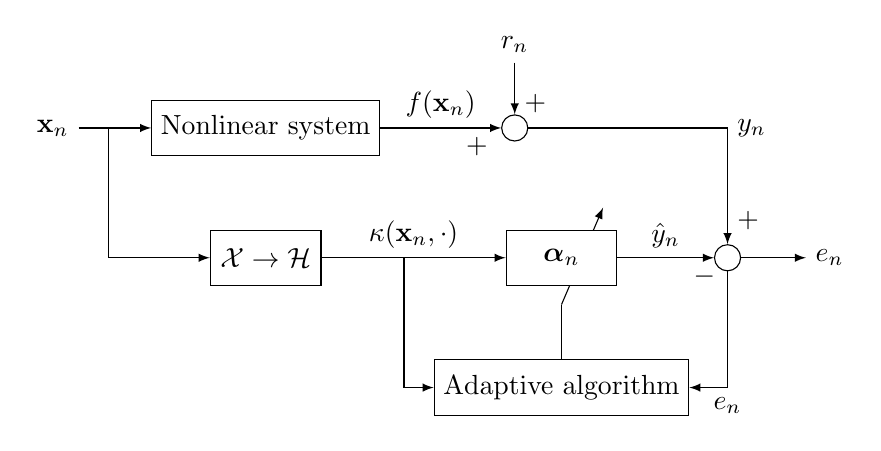
\begin{tikzpicture}[auto, node distance=2cm,>=latex]
    \node [input, name=input] {$\mathbf{x}_n$};
    \node [node, right of=input] (node1) {};
    \draw (input) -- (node1);
    \node [block, right of=node1] (system) {Nonlinear system};
    \draw [->] (node1) -- (system);
    \node [sum, right of=system, xshift=7em] (plus) {};
    \draw [->] (system) -- node[pos=0.8, below] {$+$} node {$f(\mathbf{x}_n)$} (plus);
    \node [input, name=noise, above of=plus, node distance=3em] {$r_n$};
    \draw [->] (noise) -- node[pos=0.8, right] {$+$}(plus);

    \node [block, below of=system, yshift=1em] (transformation) {$\mathcal{X}\rightarrow \mathcal{H}$};
    \draw [->] (node1) |- (transformation);
    \node [node, right of=transformation, xshift=3em] (node2) {};
    \draw (transformation) -- (node2);
    \node [block, right of=node2] (filter) {$\boldsymbol{\mathbf{\alpha}}_n$};
    \draw [->] (transformation) -- node {$\kappa(\mathbf{x}_n,\cdot)$} (filter);
    \node [sum, right of=filter, xshift=4em] (minus) {};
    \draw [->] (filter) -- node[pos=0.9, below] {$-$} node {$\hat y_n$} (minus);
    \draw [->] (plus) -| node[pos=0.9, right] {$+$} node {$y_n$} (minus);
    \node [input, right of=minus, xshift=-2em] (output) {$e_n$};
    \draw [->] (minus) -- (output);

    \node [block, below of=filter, yshift=1em] (algorithm) {Adaptive algorithm};
    \draw [->] (node2) |- (algorithm);
    \draw [->] (minus) |- node {$e_n$} (algorithm);
    \node [node, above of=algorithm, yshift=1em] (node3) {};
    \draw (algorithm) -- (node3);
    \node [node, above of=node3, xshift=1.5em, yshift=1.5em] (node4) {};
    \draw [->] (node3) -- (node4);

    \node [block, right of=node2] (filter2) {$\boldsymbol{\mathbf{\alpha}}_n$}; % repeat to fix z-index
\end{tikzpicture}
%\centerline{\includegraphics[height=150pt]{chapters/chapter_ork/fig/diagram.eps}}
\caption{Kernel-based adaptive system identification. Figure adapted from \cite{parreira2012stochastic}.}
\label{ork:fig:diagram}
\end{figure}

Online algorithms should be capable of operating during extended periods of time, processing large amounts of data. Kernel methods rely on a functional representation that grows as the amount of observations increases. A na\"ive implementation of an online kernel method will therefore require growing computational resources during operation, leading to performance issues once the available memory is insufficient to store the training data or once the computations for one update take more time than the interval between incoming data \cite{kivinen2004online}.

%%%%%%%%%%%%%%%%%%%%%%%%%%%%%%%%%%%%%%%%%%%%%%%%%%%%%%%%%%%%%%%%%%%%%

\section{Kernel adaptive filtering algorithms}

Kernel adaptive filtering algorithms are online regression algorithms. While early kernel adaptive filtering algorithms had a clear connection to classical adaptive filters, such as LMS, RLS and KAPA filters, later implementations explored Gaussian Process and projections based algorithms.

The different kernel adaptive filtering algorithms proposed in the literature vary in several aspects:
\begin{itemize}
\item The type of filter they relate to: typically LMS, RLS or KAPA;
\item The computational complexity w.r.t. the amount of elements in memory, $M$: typically $\mathcal{O}(M)$ or $\mathcal{O}(M^2)$;
\item The approach to building a sparse dictionary and to possible prune data from it afterwards;
\item The convergence speed;
\item The ability to employ multiple kernels and learn their respective weights.
\end{itemize}
The algorithm profiler described in Chapter \ref{sec:profiler} allows to compare these different aspects empirically.

\section{Algorithm code structure}

Since all algorithms share the same structure, they are coded in a common framework. In particular:
\begin{itemize}
\item Each algorithm is contained in a single file in the \verb"/lib" folder.
\item Each algorithm is implemented as an object in matlab, using the \verb"classdef" syntax.
\item Each algorithm has two basic public methods: \verb"evaluate" and \verb"train".
The object code contains only one iteration of the algorithm. The for-loop over the time index that governs the online operation should go in an external script.
\end{itemize}

Furthermore, efforts are made to make the code
\begin{enumerate}
\item As human-readable as possible, in the first place;
\item Short and structured, in the second place.
\end{enumerate}
As far as possible, algorithm structure should follow the pseudocode from the corresponding publication.

Finally, the following best practices for scientific computing are taken into account \cite{wilson2014best}:
\begin{itemize}
\item Variable naming should correspond to the nomenclature used in the corresponding publication whenever possible;
\item Comments should be used sparingly. Document the design and purpose of the code rather than its mechanics.
\end{itemize}

\section{Template for kernel adaptive filtering algorithms}

\lstinputlisting{../lib/kafbox_template.m}

\section{Performing online learning}

Each kernel adaptive filtering algorithm is implemented as a Matlab class. To perform online learning with an algorithm, first define its options:
\begin{shortlisting}
options = struct('nu',1E-4,'kerneltype','gauss','kernelpar',32);
\end{shortlisting}
Next, create an instance of the filter. E.g., for an instance of the KRLS algorithm that uses the ALD criterion run:
\begin{shortlisting}
kaf = aldkrls(options);
\end{shortlisting}
One iteration of training is performed by feeding one input-output data pair to the filter:
\begin{shortlisting}
kaf = kaf.train(x,y);
\end{shortlisting}
The outputs for one or more test inputs are evaluated as follows:
\begin{shortlisting}
Y_test = kaf.evaluate(X_test);
\end{shortlisting}

\section{Example learning script: time-series prediction}

\lstinputlisting{../demo/demo_prediction.m}

%%%%%%%%%%%%%%%%%%%%%%%%%%%%%%%%%%%%%%%%%%%%%%%%%%%%%%%%%%%%%%%%%%%%%

\chapter{Algorithm profiler}
\label{sec:profiler}

The algorithm profiler is a tool that allows to compare the trade-off between cost and performance between several algorithm configurations and/or several algorithms.

A demo configuration script is given in the file\\ \verb"demo/demo_profiler_prediction_lorenz.m".

%%%%%%%%%%%%%%%%%%%%%%%%%%%%%%%%%%%%%%%%%%%%%%%%%%%%%%%%%%%%%%%%%%%%%

\chapter{List of included algorithms}
\label{chap:algos}

Matlab implementations of the following algorithms are included in the toolbox:

\begin{itemize}
\item Approximate Linear Dependency Kernel Recursive Least-Squares (ALD-KRLS) \cite{engel2004kernel}.
\item Sliding-Window Kernel Recursive Least-Squares (SW-KRLS) \cite{vanvaerenbergh2006sliding}.
\item Naive Online Regularized Risk Minimization Algorithm (NORMA) \cite{kivinen2004online}.
\item Kernel Least-Mean-Square (KLMS) \cite{liu2008kernel}.
\item Fixed-Budget Kernel Recursive Least-Squares (FB-KRLS) \cite{vanvaerenbergh2010fixed}.
\item Kernel Recursive Least-Squares Tracker (KRLS-T) \cite{vanvaerenbergh2012kernel}.
\item Quantized Kernel Least Mean Squares (QKLMS) \cite{chen2012quantized}.
\item Random Fourier Feature Kernel Least Mean Square (RFF-KLMS) algorithm \cite{singh2012random}.
\item Extended Kernel Recursive Least Squares (EX-KRLS) \cite{liu2009extended}.
\item Gaussian-Process based estimation of the parameters of KRLS-T \cite{vanvaerenbergh2012estimation}.
\item Kernel Affine Projection (KAP) algorithm with Coherence Criterion \cite{richard2009online}.
\item Kernel Normalized Least-Mean-Square (KNLMS) algorithm with Coherence Criterion \cite{richard2009online}.
\item Recursive Least-Squares algorithm with exponential weighting (RLS) \cite{sayed2003fundamentals}.
\item Multikernel Normalized Least Mean Square algorithm with Coherence-based Sparsification (MKNLMS-CS) \cite{yukawa2012multikernel}.
\item Parallel HYperslab Projection along Affine SubSpace (PHYPASS) algorithm \cite{takizawa2013efficient}.
\item Fixed-budget kernel least mean squares (FB-KLMS) algorithm \cite{rzepka2012fixed}.
\item Leaky Kernel Affine Projection Algorithm (LKAPA, including KAPA-1 and KAPA-3) and Normalized Leaky Kernel Affine Projection Algorithm (NLKAPA, including KAPA-2 and KAPA-4) \cite{liu2008kernel}.
\item Kernel Affine Projection Subgradient Method (KAPSM) \cite{slavakis2008online}.
\item Kernel Least Mean Squares algorithm with Coherence-Sparsification criterion and L1-norm regularization (KLMS-CSL1) and with active L1-norm regularization (KLMS-CSAL1) \cite{gao2013kernel}.
\item  Mixture Kernel Least Mean Square (MxKLMS) algorithm \cite{pokharel2013mixture}.
\end{itemize}

%%%%%%%%%%%%%%%%%%%%%%%%%%%%%%%%%%%%%%%%%%%%%%%%%%%%%%%%%%%%%%%%%%%%%


\chapter{About}
\begin{itemize}
\item {\bf Name:} Kernel Adaptive Filtering Toolbox
\item {\bf Abbreviation:} KAFBOX
\item {\bf Punchline:} a Matlab benchmarking toolbox for kernel adaptive filtering
\item {\bf Author:} Steven Van Vaerenbergh
  \begin{itemize}
  \item Homepage: \url{http://gtas.unican.es/people/steven/}
  \item Email: \url{steven@gtas.dicom.unican.es}
  \item Affiliation: Advanced Signal Processing Group, Department of Communications Engineering, University of Cantabria, Spain.
  \end{itemize}
\item {\bf Collaborators:} Miguel Lazaro-Gredilla, Sohan Seth, Masahiro Yukawa, Masa-aki Takizawa, Osamu Toda, Dominik Rzepka, Pantelis Bouboulis
\item {\bf URL:} \url{https://github.com/steven2358/kafbox}
\item {\bf Citing:} Published reports of research using this code (or a modified version) should cite \cite{vanvaerenbergh2013comparative}.
\item {\bf Environment:} Matlab\footnote{\url{http://www.mathworks.com/products/matlab/}}.
\item {\bf Origin:} KAFBOX is a fork of Kernel Methods Toolbox (KMBOX) v0.6 (\url{http://sourceforge.net/p/kmbox/})
\item {\bf Extending the code:} Template files are provided to encourage external authors to include their own code into the toolbox. Contributions can be made through Github's fork and pull system.
\item {\bf License:} FreeBSD
\end{itemize}


%%%%%%%%%%%%%%%%%%%%%%%%%%%%%%%%%%%%%%%%%%%%%%%%%%%%%%%%%%%%%%%%%%%%%
%%%%%%%%%%%%%%%%%%%%%%%%%%%%%%%%%%%%%%%%%%%%%%%%%%%%%%%%%%%%%%%%%%%%%
%%%%%%%%%%%%%%%%%%%%%%%%%%%%%%%%%%%%%%%%%%%%%%%%%%%%%%%%%%%%%%%%%%%%%

\bibliographystyle{alpha}
\bibliography{kaf,extra}


\end{document}
